\subsection{Kovarians test} \label{subsec:kovarians_test}
I dette afsnit introduceres en test, der kan tildele \(p\)-værdier til prædiktorer som er udvalgt af adaptive procedurer.
Testen er baseret på LARS algoritmen og blev introduceret i \citep{lockhart}.

Betragt det velkendte lineær regression setup med en responsvariable \(\y \in \mathbb{R}^n\) og en matrix af prædiktorer \(\X \in \mathbb{R}^{n \times p}\), som er relateret ved
\begin{align}
\y = \X \beta + \boldsymbol{\epsilon}, \quad \boldsymbol{\epsilon} \sim N\del{\mathbf{0}, \sigma^2 \mathbf{I}}, \label{eq:set-up}
\end{align}
hvor \(\beta \in \mathbb{R}^p\) er ukendte koefficienter, som skal estimeres.

%For at motivere kovarians testen, vil vi først betragte forward-stepwise regression.
%Proceduren udvælger én prædiktor af gangen og vælger den prædiktor således at summen af kvadrerede residualer aftager mest.
%Lad \(\text{SSR}_k\) betegne summen af kvadrerede residualer for modellen med \(k\) prædiktorer.
%Da kan vi udlede en teststørrelse ved at betragte ændringen i SSR
%\begin{align*}
%R_k = \frac{1}{\sigma^2} \del{\text{SSR}_{k-1} - \text{SSR}_k},
%\end{align*}
%hvor \(\sigma\) antages at være kendt. 
%Denne teststørrelse følger en \(\chi_1^2\) fordeling.
%Hvis \(\sigma\) ikke er kendt, da den estimeres udfra sample variansen, hvilket resulterer i en \(F\)-test eller ækvivalent en \(t\)-test til at teste om variabel \(j\) er signifikant.
%
%Betragt forward stepwise regression: start med en tom model, tilføj en prædiktor af gangen, for hvert step vælg den prædiktor \(j\) som giver den største fald i SSR.
%Figur \ref{fig:covarians_test}(a) viser kvantilerne for \(R_1\) af forward stepwise regression imod en \(\chi_1^2\) fordeling, hvor \(\beta=0\).
%%
%\begin{figure}[H]
%\centering
% \scalebox{0.5}{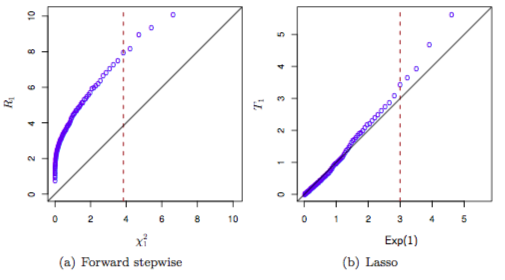
\includegraphics{fig/covarians_test.jpg}}
%\caption{Et .}
%\label{fig:covarians_test}
%\end{figure}
%%

Inden vi giver en formel beskrivelse af kovarians testen, gives en betingelse for model matricen \(\X\).
\begin{defn}[General position]
Kolonnerne \(\mathbf{X}_1, \ldots, \mathbf{X}_p\) siges at være i generel position hvis the affine span af enhver \(k+1\) vektorer \(s_1 \X_1, \ldots, s_{k+1} \X_{k+1}\) ikke indeholder ethvert element af mængden \(\cbr{\pm \X_i : \ i \neq i_1, \ldots, i_{k+1}}\) for ethvert fortegn \(s_1, \ldots, s_{k+1} \in \cbr{-1,1}\), for \(k < \min \cbr{n,p}\). 
\end{defn}
Ovenstående betingelse er svag og gælder blandt andet når indgangene af \(\X\) kommer af en kontinuert sandsynlighedsfordeling.
At kolonnerne af model matrix er i generel position sikrer at LARS og lasso stierne er entydig, som vises i \citep{lasso_unique}.

Herefter kan vi definere teststørrelsen af kovarians testen og forklare hvordan \(p\)-værdierne findes.
Vi antager det lineære regressions set-up i \eqref{eq:set-up} og at kolonner af \(\X\) er i generel position.
Vi ønsker, at teste om \(j\)'te prædiktor som er medtaget i den aktive mængde i \(\lambda_k\), dvs i \(k\)'te step af LARS algoritmen, er signifikant.
Lad \(\A_{k-1}\) betegne den aktive mængde i step \(k-1\) og lad \(\hat{\beta} \del{\lambda_{k+1}}\) være løsningen af lasso problemet i næste knot \(\lambda_{k+1}\).
Lad \(\tilde{\beta}_{\A_{k-1}} \del{\lambda_{k+1}}\) være løsningen af lasso problemet ved kun at anvende variablerne i \(\A_{k-1}\)
\begin{align*}
\tilde{\beta}_{\A_{k-1}} \del{\lambda_{k+1}} = \argmin_{\beta_{\A_{k-1}} \in \R^{\vert \A_{k-1} \vert}} \frac{1}{2n} \left\Vert \y - \X_{\A_{k-1}} \beta_{\A_{k-1}} \right\Vert_2^2 + \lambda_{k+1} \left\Vert \beta_{\A_{k-1}} \right\Vert_1,
\end{align*}
hvor \(\X_{\A_{k-1}}\) består af kolonnerne af \(\X\), som svarer til prædiktorerne i \(\A_{k-1}\).
Da kan vi definere kovarians testen
\begin{align}
T_k^\text{cov} = \frac{1}{\sigma^2} \del{ \left\langle \y, \X \hat{\beta} \del{\lambda_{k+1}} \right\rangle - \left\langle  \y, \X_{\A_{k-1}} \tilde{\beta}_{\mathcal{A}_{k-1}} \del{\lambda_{k+1}} \right\rangle}. \label{eq:6.5}
\end{align}
Intuitivt, er teststørrelsen af kovarians testen i \eqref{eq:6.5} en funktion af differensen mellem \(\X \hat{\beta}\) og \(\X_{\A_{k-1}} \tilde{\beta}_{\A_{k-1}}\), dvs de fittede værdier givet ved at medtage \(j\)'te prædiktor i den nuværende aktive mængde og undlade den.
Kovarians teststørrelsen evalueres i næste knot \(\lambda_{k+1}\), da \(j\)'te koefficient stadig er lig nul i \(\lambda_k\) og derfor
\begin{align*}
\X \hat{\beta} \del{\lambda_k} = \X_{\A_{k-1}} \hat{\beta}_{\A_{k-1}} \del{\lambda_k} = \X_{\A_{k-1}} \tilde{\beta}_{\A_{k-1}} \del{\lambda_k}
\end{align*}
Det naturlig valg for tuning parameteren i \eqref{eq:6.5} er derfor \(\lambda= \lambda_{k+1}\).
Navnet af testen kommer af at tælleren i \eqref{eq:6.5} kan skrives som differensen mellem empiriske kovarianser og et lille led.
Desto større kovarians af \(\y\) og \(\X \hat{\beta}\) sammenlignet med \(\X_{\A_{k-1}} \hat{\beta}_{A_{k-1}}\), desto vigtigere er \(j\)'te prædiktor i modellen \(\A \cup \cbr{j}\).

Under nulhypotesen at den nuværende lasso model indeholder alle sande aktive variable, som skal skrives \(\mathcal{A}_{k-1} \supseteq \text{supp} \del{\beta^*}\), hvor \(\beta^*\) er den sande koefficient vektor, da har teststørrelsen i \eqref{eq:6.5} en asymptotisk standard eksponential fordeling
\begin{align*}
T_k^\text{cov} \overset{d}{\rightarrow} \text{Exp}\del{1}.
\end{align*}
Hvis \(\sigma^2\) er ukendt, kan den estimeres under den fulde model \(\hat{\sigma}^2 = \frac{1}{n-p} \text{SSR}_p\). 
Dette indsættes i \eqref{eq:6.5}, og eksponential testen bliver en eksakt \(F_{2,n-p}\) test.

Denne test er også det naturlige analog til degrees of freedom resultaterne for lasso \eqref{eq:df_lasso} og LARS (section 2.5).
Lasso med \(k\) ikke-nul koefficienter forventes at have \(k\) frihedsgrader, og LARS anvender en frihedsgrad for hver segment \(\del{\lambda_{k+1}, \lambda_k}\) langs stien.
Kovarians testen har middelværdi lig en, som er antal frihedsgrader per trin.
%
Hernæst vil vi introducere en alternativ form af teststørrelsen i \eqref{eq:6.5}, som er nyttigt af beregningsmæssige årsager.
\begin{align*}
T_k^\text{cov} = \frac{1}{\sigma^2} \omega_k^2 \cdot \lambda_k \del{\lambda_k - \lambda_{k+1}},
\end{align*}
hvor \(\lambda_k\) og \(\lambda_{k+1}\) er LARS knots i step \(k\) og \(k+1\) af stien og \(\omega_k\) er vægten givet i \eqref{eq:post_42}.


%
%Hvis \(\X\) er ortogonal, da er teststørrelsen for kovarians testen givet ved
%\begin{align*}
%T_k^\text{cov} = \frac{1}{\sigma^2} \lambda_k \del{\lambda_k - \lambda_{k+1}}
%\end{align*} 
%Derudover fandt vi at \eqref{eq:ortogonal_lasso} som også kan skrives \(\hat{\beta}_j = S_\lambda \del{\frac{1}{n} \mathbf{x}_j^T \y}\).
%Lad \(\mathbf{U}_j = \mathbf{x}_j^T \y\) for \(j=1,\ldots, p\). 
%Knots i lasso stien er blot værdierne af \(\lambda\) for hvilket koefficienterne er ikke-nul
%\begin{align*}
%\lambda_1 = \vert \mathbf{U}_{(1)} \vert, \quad \lambda_2 = \vert \mathbf{U}_{(2)} \vert, \quad \ldots, \lambda_p = \vert \mathbf{U}_{(p)} \vert, \quad,
%\end{align*}
%hvor \(\vert \mathbf{U}_{(1)} \vert \geq \vert \mathbf{U}_{(2)} \vert \geq \dots \geq \vert \mathbf{U}_{(p)} \vert\) er order statistics af \(\vert \mathbf{U}_1 \vert, \ldots, \vert \mathbf{U}_p \vert\).
%Derfor 
%\begin{align*}
%T_k^\text{cov} = \frac{1}{\sigma^2}  \vert \mathbf{U}_{(k)} \vert \del{ \vert \mathbf{U}_{(k)} \vert -  \vert \mathbf{U}_{(k+1)} \vert}
%\end{align*}


Kovarians testen har nogle begrænsninger.
Først skal der gælde en betingelse for model matricen \(\X\).
Hvis der eksisterer en kategorisk variabel blandt prædiktorerne, og den resulterende variabel beskrives af dummy variable, da er antagelse om at kolonnerne af \(\X\) er i general position altså ikke overholdt.
Derudover tager testen ikke højde for, hvis nogle variable medtages i modellen mere end én gang (som er tilladt for lasso modificeringen af LARS algoritmen), da behandles hver situation separat og testene udføres separat.
Til sidst er testen kun asymptotisk.

I næste afsnit introduceres en test som kan anvendes efter modeludvælgelse og som giver en eksakt fordeling af teststørrelsen.